\subsubsection{2.5. Kết quả kiểm thử trên mô hình CNN + MGAT + mô hình phân lớp truyền thống với toàn bộ phương thức}
\indent\indent Nhằm đánh giá một cách khách quan chất lượng của các đặc trưng (features) được học bởi kiến trúc đồ thị, đề tài tiến hành thực hiện một thực nghiệm bổ sung, trong đó bộ phân lớp học sâu (FastKAN/MLP) được thay thế bằng các thuật toán máy học truyền thống.\vspace{0.3cm}

Đối với các mô hình máy học truyền thống, quá trình huấn luyện được thực hiện trên các đặc trưng đã được trích xuất sẵn từ mô hình học sâu, bằng cách dùng mô hình CNN backbone + MGAT + FastKAN/MLP đạt kết quả kiểm thử tốt nhất được sử dụng làm bộ mã hóa bằng cách loại bỏ tầng phân lớp cuối cùng. Vector đặc trưng đại diện cho mỗi mẫu đồ thị được xây dựng bằng cách lấy trung bình các vector đặc trưng của toàn bộ các đỉnh thành phần, từ đó thu được một vector đặc trưng có số chiều là 512. Trước khi đưa vào huấn luyện, các vector đặc trưng này được chuẩn hóa bằng kỹ thuật \textit{StandardScaler} nhằm giảm thiểu sự chênh lệch về độ lớn giữa các chiều, giúp các thuật toán máy học truyền thống hoạt động ổn định và hiệu quả hơn. Sáu mô hình máy học truyền thống được lựa chọn để đánh giá bao gồm: KNN, Naive Bayes, Decision Tree, Random Forest, Logistic Regression và Linear SVC.\vspace{0.3cm}

\newpage
Bảng số liệu và các biểu đồ dưới đây trình bày kết quả kiểm thử trung bình của các mô hình máy học truyền thống:
\begin{table}[H]
\centering
\caption{\centering Kết quả kiểm thử trung bình của các mô hình truyền thống (sử dụng đặc trưng từ DenseNet121 + MGAT + FastKAN)}
\label{tab:TraditionalModelsSummary}
\renewcommand{\arraystretch}{1.15}
\begin{tabular}{lcccc}
\hline
\textbf{Mô hình} & \textbf{Accuracy} & \textbf{Precision} & \textbf{Recall} & \textbf{F1-Score} \\
\hline
KNN (k = 1)                   & 0.8213 & 0.8289 & 0.8213 & 0.8022 \\
Gaussian NB                   & 0.7306 & 0.7210 & 0.7306 & 0.7142 \\
Decision Tree (max\_depth = 10) & 0.7556 & 0.7656 & 0.7556 & 0.7412 \\
Random Forest (n\_estimators = 20) & 0.8083 & 0.8108 & 0.8083 & 0.7859 \\
Logistic Regression (C = 10)      & 0.8370 & 0.8419 & 0.8370 & 0.8272 \\
Linear SVC (C = 0.01)             & 0.8676 & 0.8696 & 0.8676 & 0.8649 \\
\hline
{DenseNet121 + MGAT + FastKAN} & \textbf{0.9435} & \textbf{0.9477} & \textbf{0.9435} & \textbf{0.9438} \\
\hline
\end{tabular}
\end{table}

\begin{figure}[H]
    \centering
    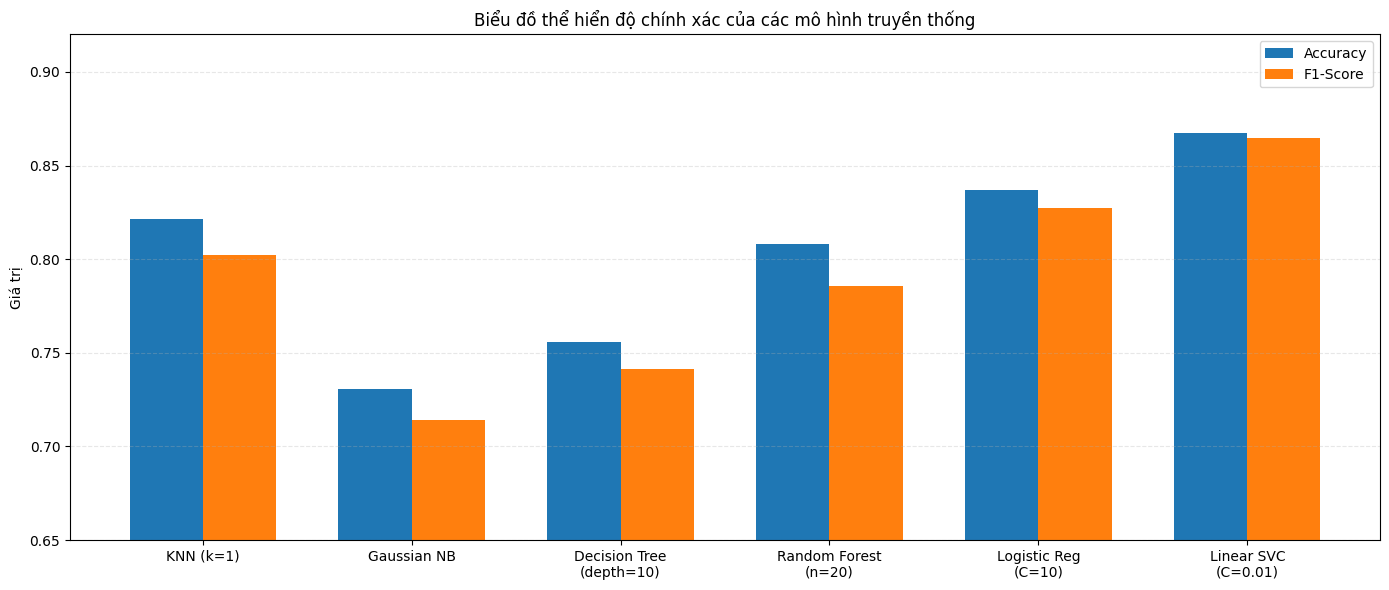
\includegraphics[width=\linewidth]{images/part-02/chap-03/sec-02/Tradition.png}
    \caption{\centering Biểu đồ thể hiện kết quả kiểm thử trung bình của các mô hình truyền thống (sử dụng đặc trưng từ DenseNet121 + MGAT + FastKAN)}
    \label{fig:KQTradition}
\end{figure}

\indent Dựa trên số liệu thu được từ bảng kết quả kiểm thử trung bình của các mô hình máy học truyền thống, có thể rút ra một số nhận xét chính như sau:\vspace{-0.1cm}
\begin{itemize}[label={--}, itemsep=1pt]
    \item Khả năng phân tách tuyến tính của không gian đặc trưng: Kết quả đạt được với Linear SVC (độ chính xác 0.8676) cho thấy các vector đặc trưng đầu ra từ tầng MGAT có mức độ phân tách tuyến tính tương đối tốt. Điều này cho thấy các mẫu dữ liệu cùng lớp có xu hướng được gom cụm trong không gian đặc trưng, tạo điều kiện thuận lợi cho các bộ phân lớp tuyến tính hoạt động hiệu quả.
    
    \item Vai trò trích xuất và tổng hợp đặc trưng của MGAT: Các kết quả kiểm thử đã cho thấy rằng kiến trúc MGAT tổng hợp thông tin từ nhiều phương thức dữ liệu rời rạc (hình ảnh, văn bản và âm thanh) thành các vector biểu diễn ngữ nghĩa thống nhất rất hiệu quả, trước khi được đưa vào các bộ phân lớp ở giai đoạn cuối.
    
    \item So sánh với FastKAN: Mặc dù Linear SVC cho kết quả khả quan, vẫn còn tồn tại một khoảng cách đáng kể về độ chính xác (khoảng 7–8\%) khi so sánh với FastKAN (đạt 0.9435). Sự chênh lệch này thể hiện hạn chế của các mô hình tuyến tính trong việc xử lý các biên quyết định phức tạp. Đối với dữ liệu ICH, nơi tồn tại nhiều mẫu có mức độ nhập nhằng cao, các bộ phân lớp phi tuyến với khả năng biểu diễn linh hoạt như FastKAN sẽ phù hợp hơn so với các mô hình máy học truyền thống.
\end{itemize}